% -*- Mode:TeX -*-
% LaTeX template for CinC papers                   v 1.1a 22 August 2010
%
% To use this template successfully, you must have downloaded and unpacked:
%       http://www.cinc.org/authors_kit/papers/latex.tar.gz
% or the same package in zip format:
%       http://www.cinc.org/authors_kit/papers/latex.zip
% See the README included in this package for instructions.
%
% If you have questions, comments or suggestions about this file, please
% send me a note!  George Moody (george@mit.edu)
%
\documentclass[twocolumn]{cinc}
\usepackage{graphicx}
\begin{document}
\bibliographystyle{cinc}

% Keep the title short enough to fit on a single line if possible.
% Don't end it with a full stop (period).  Don't use ALL CAPS.
\title{Quantum Semiprime Factorization: Leveraging Grover's Algorithm for Efficient Prime Decomposition}

% Both authors and affiliations go in the \author{ ... } block.
% List initials and surnames of authors, no full stops (periods),
%  titles, or degrees.
% Don't use ALL CAPS, and don't use ``and'' before the name of the
%  last author.
% Leave an empty line between authors and affiliations.
% List affiliations, city, [state or province,] country only
%  (no street addresses or postcodes).
% If there are multiple affiliations, use superscript numerals to associate
%  each author with his or her affiliations, as in the example below.

% \author {Jacob Collins$^{1}$, Jaime Raigoza$^{1}$, Sam Siewert$^{1}$ \\
\author{Jacob Collins$^{1}$, Jaime Raigoza$^{1}$, Sam Siewert$^{1}$ \\
\ \\ % leave an empty line between authors and affiliation
 $^1$ California State University, Chico, United States (note- full address at end of paper)}

\maketitle

% LaTeX inserts the ``Abstract'' heading in the proper style and
% sets the text of the abstract in italics as required.
\begin{abstract}

  In quantum computing, SP (semiprime) factoring is typically performed 
  with Shor's algorithm, but it is possible to achieve the same results
  more efficientily via Grover's algorithm\cite{quantum_factoring, grover}. 

  Key terms: Semiprime, superposition, entanglement, RSA encryption, (add more).

  The abstract with its heading should not be more than 100 mm long,
  which is equivalent to 25 lines of text. Leave 2 line spaces at the
  bottom of the abstract before continuing with the next heading.


\end{abstract}
% LaTeX inserts the extra space here automatically.

\section{Introduction}

The practicality of applied quantum computing is a topic of much debate,
and there are not many examples of quantum computers being able to out-perform
their classical counterpart, yet.

Quantum algorithms have been in development at a theoretical level for
decades, but the application of these methods is still in early stages.
It is quite common to find code which implements a quantum algorithm like
Grover's or Shor's, but very often these programs are hard-coded, and only
work for a small handful of specific values\cite{shors_ibm}.

Include a figure of our circuit diagram and briefly describe what it 
does, and how it does it.

  \subsection{Motivation}

  Why are we replicating the research, why is this important.

  Quantum computers are a technology very much still under development. 
  As such, one of the major limitations for applied quantum computing is 
  the number of qubits required to perform a given task. If it can be verified 
  that SP factoring with Grover's algorithm uses significantly less qubits than
  Shor's, then the application of these techniques will be feasible far sooner.

  \subsection{Semiprime Factoring}  

  What is SP factoring and why is it important. RSA, etc.

\section{Goals}

The goal of this research endeavor is to estimate the problem scaling point
at which some quantum algorithm may be able to out-perform our best classical
solution to the same problem.

Grover's algorithm has an incredibly wide range of potential use-cases,
and an intention for this paper is to provide a generalized reference
for how Grover's algorithm may be used to invert a given function.

\section{Literature Review}

  \subsection{Grover's Algorithm}

  Grover's Algorithm is a quantum computing method 
  that can be used to search a database of $n$ values in $O(\sqrt{n})$ time 
  rather than the naive classical time complexity of $O(n)$\cite{grover}. 

  The exact number of iterations required varies on a case-by-case basis,
  but is typically expressed as follows: in a search for one matching input
  state, $\frac{\pi}{4}\sqrt{N}$ iterations are required, and in a search
  for $k$ valid input states, $\sqrt{\pi}{4}\cdot \sqrt{\frac{N}{k}}$
  iterations are required, where $N$ is the size of the search domain.

  In most cases, $N=2^n$, where $n$ is the number of bits needed to represent
  the target value. This is by no means a steadfast rule, and is meant as 
  a helpful starting point for any confused readers attempting to implement
  something similar themselves.
  
  Given a function $f(x)=y$, where $x$ is unknown (index, prime factors, 
  sum components, etc.), and $y$ is known (array value, semiprime/product, 
  sum, etc.), Grover's algorithm effectively takes the role of $f'(y)=x$, 
  allowing for a potential speedup in finding whatever input (s) to $f(x)$
  will return $y$, provided that it is much faster to compute $f(x)$ than
  whatever classical methods might be used to otherwise solve for $x$ given $y$.

  This speedup comes from the fact that Grover's algorithm requires 
  $O(\sqrt{y})$ iterations, each of which have a time complexity proportional
  to that of $f(x)$.

  \subsection{Shor's Algorithm}

  Shor's algorithm is the most well-known approach to prime factorization
  in quantum computing. However, there are many drawbacks to this approach,
  the most notable of which being the need to take measurements mid-circuit
  and essentially re-run with new values afterwards, which introduces a 
  significant amount of overhead. Even recently improved versions of Shor's
  algorithm still require a minimum of $2n+1$ qubits, and tend to be 
  extremely sensitive to noise, which leads to high error\cite{quantum_factoring,shor}.

  Furthermore, when it comes to more concrete applications of Shor's algorithm,
  a full-scale implementation of this algorithm to factor an $n$-bit number
  may require up to $5n+1$ qubits for accurate results, and require 
  on the order of $n^3$ operations~\cite{quantum_fac_efficient}.

  \subsection{Quantum Factoring Algorithm with Grover Search}

  S. Whitlock, et al.\ present a method of SP factoring with Grover's
  algorithm. The implementation in their paper is highly optimized,
  and modifies the target value in their circuit from some semiprime $N$,
  to $M$, a reduced number uniquely tied to $N$, which has unique factors 
  $p$ and $q$ which can be used to calculate $a, b$, the prime factors of 
  $N$. This optimization from $N$ to $M$ allows the implementation to ignore
  the trivial prime factors $2$ and $3$, and requires fewer qubits than would
  otherwise be needed to search for prime factors of $N$~\cite{quantum_factoring}.

  While this approach is admirable, it introduces a level of complexity 
  that may hinder a learner's understanding of the mechanics at work,
  so the implementation shown in section\ \ref{sec:Methodology} forgoes
  this abstraction from $N$ to $M$, and instead implements an oracle which
  searches directly for prime factors $a$ and $b$ of a semiprime $N$.

\section{Methodology}\label{sec:Methodology}

\begin{figure*}[!ht]\label{fig:FIGURA1}
\centering
% 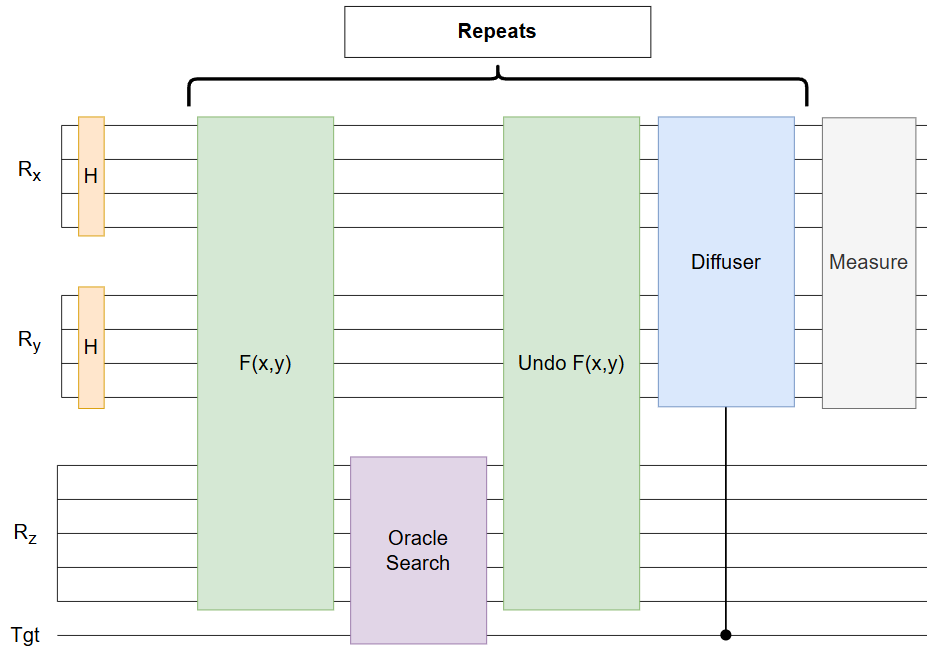
\includegraphics[width=7.9cm]{grover_inversion.png}
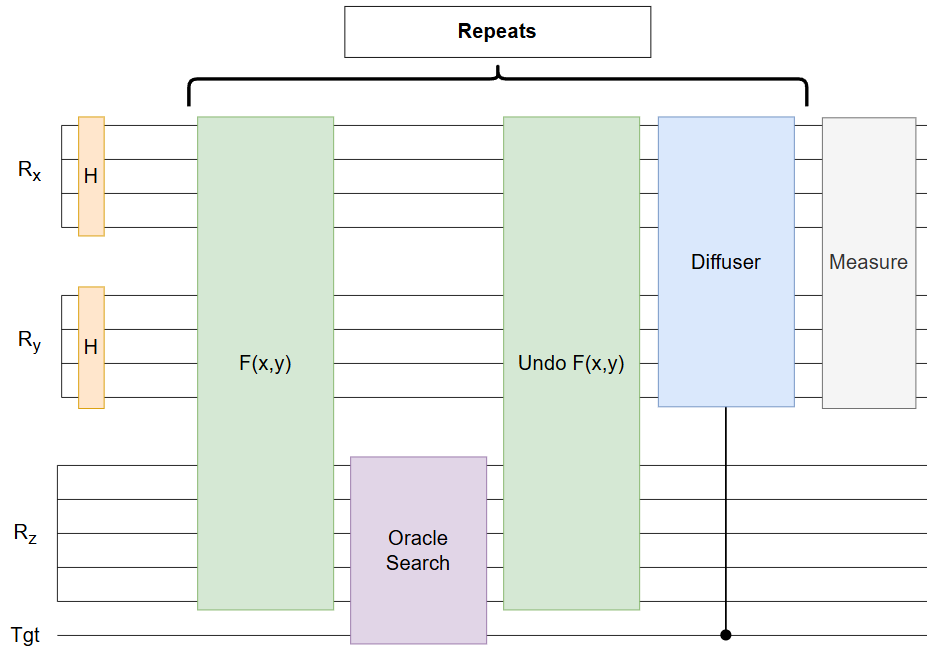
\includegraphics[width=15.8cm]{grover_inversion.png}
\caption{General circuit diagram for Grover's Algorithm, used to find 
the inputs $x, y$ for which $f(x,y)=z$, for some known output $z$.}
\end{figure*}

Quantum algorithms take advantage of superposition and entanglement,
which enables many methods of computation which are otherwise impossible
with a classical computer. For example, by placing a set of $n$ qubits 
(otherwise known as a qubit \textbf{register}) in superposition, that register
simultaneously represents every value which can be represented in $n$ bits,
until measured. Once measured, a register in uniform superposition will 
collapse into one of these states with equal likelihood.

In a given register $R_n$ with $n$ qubits, values are represented in binary,
such, for example, if some number $N=3$ were to be represented classically
with $n=4$ bits, it might be seen in binary as $0011$, and on a qubit
register that number may be represented similarly as $| 0011 \rangle$.

  \subsection{Grover's Algorithm for General Function Inversion} 

  Operations can be performed on a set of input registers that start in uniform 
  superposition, and these operations will affect each potential state individually. 
  The properties of superposition are utilized by Grover's Oracle to selectively 
  modify the states $|x,y\rangle$ in the input registers $R_x$ and $R_y$,
  marking them as valid by setting them to $-|x,y\rangle$, only when the output register
  $R_z$ matches some known search term $z$. An outline of a quantum circuit for
  Grover's algorithm is seen in Figure~\ref{fig:FIGURA1}.

  The oracle in Grover's algorithm performs a controlled operation which is meant
  to differentiate states $x,y$ that do result in the wanted target $z$ from 
  states $x,y$ that do not result in the target $z$.
  
  \begin{figure}[h]\label{fig:FIGURA2}
  \centering
  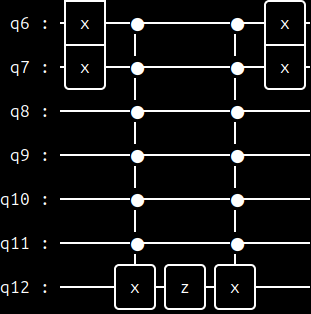
\includegraphics[width=6.0cm]{oracle_15.png}
  % 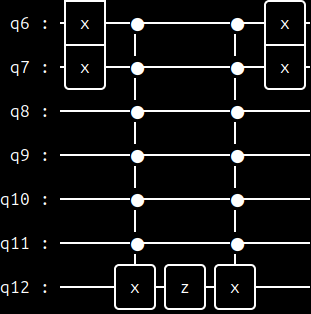
\includegraphics[width=7.9cm]{oracle_15.png}
  \caption{Example circuit diagram for Grover's oracle marking states of the input
  registers $R_x$ and $R_y$ ($[q_0,q_2]$ and $[q_3,q_5]$, respectively) which
  result in $z=15$.}
  \end{figure}

  Figure~\ref{fig:FIGURA2} shows an example of the oracle searching for the state $z=15$,
  or rather, $R_z=|001111\rangle$. To implement a circuit which can selectively target
  $z=15$, Toffoli gates (otherwise known as NOT, or X gates) are applied on 
  $R_z[0]$ and $R_z[1]$, so that states where $R_z=|001111\rangle$ will temporarily be in
  state $R_z=|111111\rangle$, and the multi-controlled Toffoli gates\cite{multi_toffoli}
  will apply only for the desired states. These operations are then performed again,
  returning all but the target qubit (which has the Z-gate applied) to their original
  states.

  \begin{figure}[h]\label{fig:FIGURA3}
  \centering
  % 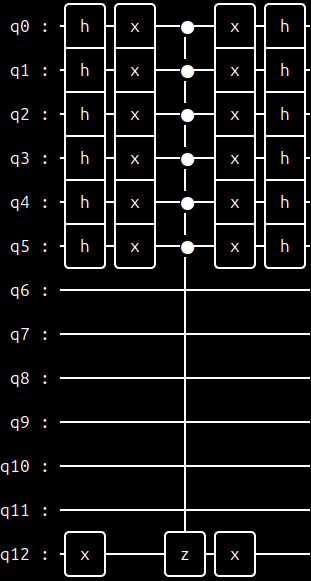
\includegraphics[width=7.9cm]{diffuse.png}
  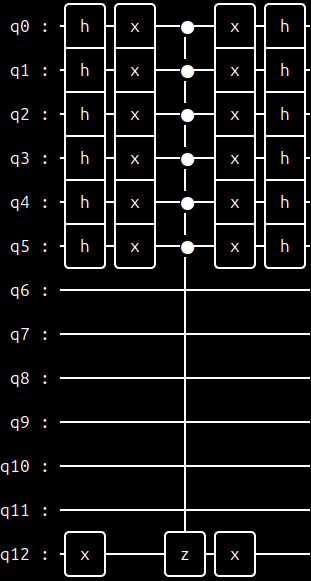
\includegraphics[width=5.0cm]{diffuse.png}
  \caption{Example circuit diagram for a diffuser which amplifies the probability that
  measurement will result in a state which has been marked by the oracle.
  Input registers $R_x$ and $R_y$ (q0-q2 and q3-q5, respectively) after diffusion are 
  more likely to be measured in a state such that $f(R_x,R_y)$ results in $R_z=|z\rangle$.}
  \end{figure}

  The diffuser in Grover's algorithm (Figure~\ref{fig:FIGURA3}) can then increase the 
  probability of observing $-|x,y\rangle$ (states which have been marked by the oracle) 
  through a process known as inversion about the mean.

  \subsection{Semiclassical Arithmetic} 

  As a proof of concept (prior to the release of~\cite{quantum_factoring}),
  a function $f(x,y)=x+y$ is defined such that $R_x=|x\rangle$, $R_y=|y\rangle$,
  and after performing $f(R_x,R_y)$, the output register $R_z$ shall be in the
  state $|x+y\rangle$.
  
  This approach was implemented in a similar manner to a classical full-adder,
  and worked on quantum simulators with $100\%$ accuracy~\cite{quantum_full_adder}.

  The semiclassical full-adder indeed works with Grover's algorithm, states were
  filtered to only measure inputs which resulted in a sum matching some given value.
  This is a trivial problem however, and only has potential usefulness due to the 
  relationship between multiplication and addition.

  Semiclassical arithmetic does have significant drawbacks, however. Despite
  being relatively simple to implement due to the similarity with principles
  that have a much broader range of documentation, the classical nature of this
  implementation meant that in order to move to multiplication from this point,
  the value of one register would need to be measured, and $R_x$ would then be
  added to $R_z$ a number of times dependent on the value of $y$.

  Measuring the state of either input register would collapse the superposition,
  and break the underlying principles on which Grover's algorithm depends. Thus,
  a different approach became necessary- one that could bridge the gap between 
  addition and multiplication without needing to measure either register,
  so that the operation can still work with inputs that are in superposition,
  allowing the use of Grover's algorithm.

  \subsection{Arithmetic in the Quantum Fourier Domain}  

  Describe the updated methods of quantum arithmetic, and how it solved the 
  previous problems.

  Figures to visualize how the weighted phase shifts work to produce
  expected results matching addition, scaled addition, and register 
  multiplication.

\section{Results and Discussion}

Include some charts showing our runtime and qubit requirements vs N.

  \subsection{Accuracy and Limitations}

  How precise and accurate were our measurements. Mention edge-cases like
  square semiprimes, etc.

  How many qubits were we able to simulate, i.e., how large of semiprimes
  can we factor with our current systems.

  \subsection{Comparison to Shor's Algorithm}

  List strengths and weaknesses of Shor's, i.e., more documentation, more
  examples, larger code base to reference, but ours is faster and uses less
  qubits.

\section{Conclusion}

What have we learned so far, what does it mean, at what problem scale might
we see quantum advantage based on our results, etc.

\section{Future Work}
 
Implementation of the optimization with M, S, p, and q, rather than just 
a and b from N.

\section*{Acknowledgments}  
% This section is not numbered.
% 
Acknowledge the source paper.


% LateX generates the ``References'' heading automatically and switches
% to 9 point type for the bibliography.  Please  use BibTeX and
% follow the examples in the sample 'refs.bib' file to enter your references.
\bibliography{refs}

% If you don't use BibTeX (why not?) , comment out or remove the previous
% line, and uncomment the following lines up to the ``}\end{bibliography}''
% line below:
%\begin{thebibliography}{99}{ %\small
% \bibitem{tag} (General form) J. K. Author, ``Name of paper,''
%   \emph{Abbrev. Title of
%   Periodical}, vol. x, no. x, pp. xxx--xxx, Abbrev. Month, year. 

% \bibitem{ito}  M. Ito et al., ``Application of amorphous oxide TFT to
%   electrophoretic display,'' \emph{J. Non-Cryst. Solids}, vol. 354, no. 19,
%   pp. 2777--2782, Feb. 2008.
  
% \bibitem{fardel}  R. Fardel, M. Nagel, F. Nuesch, T. Lippert, and
%   A. Wokaun, ``Fabrication of organic light emitting diode pixels by
%   laser-assisted forward transfer,'' \emph{Appl. Phys. Lett.}, vol. 91,
%   no. 6, Aug. 2007, Art. no. 061103.
  
% \bibitem{buncombe} J. U. Buncombe, ``Infrared navigation Part I: Theory,''
%     \emph{IEEE Trans. Aerosp. Electron. Syst.}, vol. AES-4, no. 3,
%     pp. 352--377, Sep. 1944.
      
% Uncomment the following line if you are not using BibTeX.
%}\end{thebibliography}


% LaTeX inserts the ``Address for correspondence'' heading.
\begin{correspondence}
Jacob Collins\\
1565 Filbert Ave\\
jbcollins@csuchico.edu
\end{correspondence}

\balance

\end{document}

